\section{Spezielle Relativitätstheorie}%
\label{srel:sec:spezielle_relativitaetstheorie}

\begin{itemize}
	\item \textbf{Relativität}: Zeit- und Raumangaben sind von einem fest gewählten \textbf{Bezugssystem} abhängig, physikalische Gesetze sind durch Bezugssysteme bedingt
\end{itemize}

\subsection{Michelson-Morley Experiment}%
\label{srel:sub:michelson_morley_experiment}

\begin{minipage}{0.5\textwidth}
	\begin{center}
		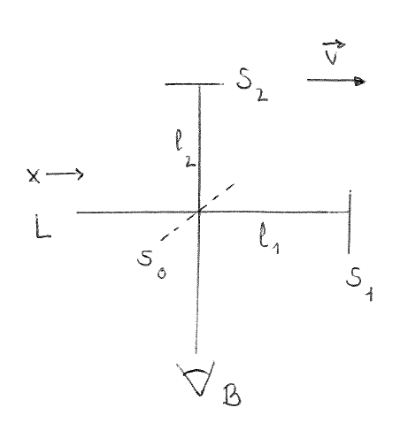
\includegraphics[width=0.7\textwidth]{images/michelson-morley.png}
	\end{center}	
\end{minipage}
\begin{minipage}{0.5\textwidth}
	\begin{itemize}
		\item Lichtquelle $L$
		\item Beobachter $B$
		\item Halbdurchlässiger Spiegel $S_0$
		\item Spiegel $S_1, S_2$
		\item Driftgeschwindigkeit $\vec{v}$
	\end{itemize}
\end{minipage}

\begin{itemize}
	\item \textbf{Idee}:
	\begin{itemize}
		\item Licht breitet sich im gesamten Universum aus, Äther (Lichtmedium) sollte dann auch das Universum einnehmen (\quotestyle{Weltäther})
		\item Erde driftet um die Sonne, somit auch durch den Äther
		\item \textbf{Frage 1.}: Breitet sich Licht zu verschiedenen Jahreszeiten unterschiedlich aus?
		\item \textbf{Frage 2.}: Kann man die Geschwindigkeit der Erde relativ zum Äther bzw. des Äthers relativ zur Sonne ermitteln?
		\item \textbf{Beobachtung 1.}: Interferenzstreifen beim Beobachter, abhängig von unterschiedlichen Laufzeiten des Lichtes
		\item \textbf{Beobachtung 2.}: Keine Interferenzverschiebung nach Drehen und Verstellen des Apparates
	\end{itemize}
	\item \textbf{Folgerungen}:
	\begin{itemize}
		\item Lichtgeschwindigkeit ist \textbf{überall gleich}
		\item Es gibt weder \textbf{absolute Zeit} noch \textbf{absoluten Raum}
		\item Galilei-Transformation muss falsch sein, wenn es weiter Interferenzsysteme geben soll
		\item Begriff der \textit{Gleichzeitigkeit} ist an die Synchronisation mittels Licht geknüpft
	\end{itemize}
\end{itemize}

\subsection{Einsteinsche Postulate}%
\label{srel:sub:einsteinsche_postulate}

\begin{itemize}
	\item \textbf{Relativitätsprinzip}: \itquote{Die Form der physikalischen Gesetze bleibt in jedem Inertialsystem gleich.}
	\item \textbf{Konstanz der Lichtgeschwindigkeit}: \itquote{Die Lichtgeschwindigkeit im Vakuum ist in allen Inertialsystemen gleich (d.h. unabhängig von der Bewegung der Quellen).}
\end{itemize}

\newpage
\subsection{Lorentztransformation}%
\label{srel:sub:lorentztransformation}

\begin{itemize}
	\item \textbf{Koordinatentransformation} zur Beschreibung von Phänomenen in verschiedenen \textbf{Bezugssystemen}
	\item \textbf{Ereignis}: Etwas, das in Raum und Zeit lokalisiert ist; lässt sich mit einem \textbf{Vierervektor} ausdrücken:
	$$
		x = (x^0, x^1, x^2, x^3) = (ct, \vec{r}) = (ct, x, y, z)
	$$
	\item Vierervektoren sind Elemente des \textbf{Minkowski-Raumes}, der zur eleganten Formulierung der Relativitätstheorie dient
	\item \textbf{Index-Notation}:
	\begin{itemize}
		\item \textbf{Einsteinsche Summenkonvention}: Weglassen von Summenzeichen, es wird über doppelt auftretende Indizes summiert, z.B bei Matrixmultiplikation:
		\begin{align*}
			(A \cdot B)_{ij} = \sum^n_{k=1}A_{ik} \cdot B_{kj} \Leftrightarrow (A \cdot B)_{ij} = A_{ik} \cdot B_{kj}
		\end{align*}
		\item Komponenten von Vierervektoren erhalten griechische Indizes und sind je nach Position des Index entweder
		\begin{itemize}
			\item \textbf{Kontravariant}: $x^\mu = (ct, \vec{x})$
			\item \textbf{Kovariant}: $x_\mu = (ct, -\vec{x})$
		\end{itemize}
	\end{itemize}
	\item Die \textbf{Allgemeine Lorentztransformation} ist gegeben durch die \textbf{Spezielle Lorentztransformation} multipliziert mit einer \textbf{Drehung}
	\item Die \textbf{Spezielle Lorentztransformation} transformiert zwischen zwei Beobachtern mit unterschiedlicher, konstanter Geschwindigkeit
	\item \textbf{Transformationsmatrix} $\mathbf{L}$:
	$$
		L =
		\begin{pmatrix}
			\gamma & 0 & 0 & \gamma\beta\\
			0 & 1 & 0 & 0\\
			0 & 0 & 1 & 0\\
			-\gamma\beta & 0 & 0 & \gamma
		\end{pmatrix}
		=
		\begin{pmatrix}
			cosh\ y & 0 & 0 & -sinh\ y\\
			0 & 1 & 0 & 0\\
			0 & 0 & 1 & 0\\
			-sinh\ y & 0 & 0 & cosh\ y
		\end{pmatrix}
	$$
	$$
			\beta = \frac{v}{c},\ \gamma = \frac{1}{\sqrt{1 - \beta^2}},\ \vec{x} = \begin{pmatrix}ct\\\vec{v}\end{pmatrix},\ y = tanh^{-1}\frac{v}{c}
	$$
	\item \textbf{Folgerungen}:
	\begin{itemize}
		\item \textbf{Zeitdilatation}: $\Delta t' = \gamma\Delta\tau$ (\textbf{Eigenzeit} $\Delta\tau$: Zeit, die in einem Bezugssystem verstreicht, in dem alle Ereignisse am selben Ort stattfinden)
		\item \textbf{Längenkontraktion}: $l' = \frac{l_0}{\gamma}$ (\textbf{Eigenlänge} $l_0$: Länge eines Objektes in einem Bezugssystem, in dem es sich in Ruhe befindet)
		\item \textbf{Relativistische Geschwindigkeitsaddition}: $\beta_3 = \frac{\beta_1 + \beta_2}{1 + \beta_1\beta_2}$ bzw. $cosh\ \eta_3 = cosh(\eta_1 + \eta_2)$
	\end{itemize}
\end{itemize}

\subsection{Relativistische Mechanik}%
\label{srel:sub:relativistische_mechanik}

\begin{itemize}
	\item \textbf{Relativistische Geschwindigkeit}: $$u^\mu = \frac{dx^\mu}{d\tau} = \gamma(c, \vec{v})$$
	\item \textbf{Relativistischer Impuls}: (\textbf{Gesamtenergie des Teilchens} $\mathbf{E}$, \textbf{Ruhemasse} $\mathbf{m}$) $$p^\mu = mu^\mu = (\gamma m c, \gamma m \vec{v}) = (\frac{E}{c}, \gamma m \vec{v})$$
	\item \textbf{Relativistische Kraft}: $$K^\mu = m\frac{du^\mu}{d\tau} = \gamma \begin{pmatrix}\frac{\vec{F}\vec{v}}{c}\\\vec{F}\end{pmatrix}$$
\end{itemize}